\chapter{Технологический раздел}
\label{cha:impl}

%В данном разделе обоснован выбор средств разработки приложения, представлены детали разработки и дается описание презентационного уровня приложения.

\section{Выбор средств разработки}

В качестве системы управления базами данных была выбрана PostgreSQL\cite{postgres}, поскольку данная СУБД поддерживает необходимую модель данных, выбор которой был обоснован ранее, также эта СУБД является свободным программным обеспечением (open source) и является бесплатной.

В качестве языка программирования для написания серверной части приложения был выбран Golang\cite{golang}, поскольку он поддерживает все необходимые инструменты для решения поставленной задачи: предоставляется функционал для написания простых одностраничных серверов и http-клиентов, также он предоставляет необходимые инструменты для взаимодействия с БД, созданной с использованием PostgreSQL. 

В ходе решения поставленной задачи были использованы дополнительные инструменты, расширяющие базовый функционал языка Golang: gorilla/mux\cite{golang} для настройки маршрутизации, http\cite{http} для обработки входящих и исходящих запросов, sessions\cite{sessions} для управления сессией пользователя, пакет pq\cite{pq} для взаимодействия с БД. Для шифрования данных был использован пакет x/crypto\cite{crypto}, для валидации данных - go-ozzo/validation\cite{validation}.

Для оформления клиентских страниц веб-сервера был использован язык разметки HTML/CSS\cite{html}.

\clearpage

\section{Детали разработки приложения}

\subsection*{Описание структур, соответствующих таблицам базы данных}

В данном разделе представлены структуры, описывающие таблицы базы данных. Структурам Admin, Doctor и Patient дополнительно создано поле Encrypted\_password с целью хранения зашифрованного пароля.

На листингах 3.1-3.2 представлены структуры, соответствующие таблицам из базы данных.

\begin{lstlisting}[caption={Структуры, описывающие таблицы из базы данных}]
type Admin struct {
	ID                int    `json:"id"`
	Name		      string `json:"name"`
	Surname           string `json:"surname"`
	Email             string `json:"email"`
	Password          string `json:"password,omitempty"`
	EncryptedPassword string `json:"-"`
}

type Doctor struct {
	ID                int    `json:"id"`
	Name		      string `json:"name"`
	Surname           string `json:"surname"`
	Work_since        int    `json:"work_since"`
	Spec_id           int    `json:"spec_id"` 
	Email             string `json:"email"`
	Password          string `json:"password,omitempty"`
	EncryptedPassword string `json:"-"`
}

type Patient struct {
	ID                int    `json:"id"`
	Name		      string `json:"name"`
	Surname           string `json:"surname"`
	Gender            string `json:"gender"`
	Birth_year        int    `json:"birth_year"`
	Phone             string `json:"phone"`
	Email             string `json:"email"`
	Password          string `json:"password,omitempty"`
	EncryptedPassword string `json:"-"`
}
\end{lstlisting}
\clearpage
\begin{lstlisting}[caption={Структуры, описывающие таблицы из базы данных (продолжение)}]
type Disease struct {
	ID                int    `json:"id"`
	Name		      string `json:"name"`
	Spec_id           int    `json:"spec_id"`
}

type Specialization struct {
	ID     int    `json:"id"`
	Name   string `json:"name"`
	Salary int    `json:"salary"`
}

type Medicine struct {
	ID   int    `json:"id"`
	Name string `json:"name"`
	Cost int    `json:"cost"`
}

type Visit struct {
	ID                int    `json:"id"`
	Status            string `json:"status"`
	Doctor_id         int    `json:"doctor_id"`
	Patient_id        int    `json:"patient_id"`
}

type Record struct {
	ID          int    `json:"id"`
	Visit_id    int    `json:"visit_id"`
	Disease_id  int    `json:"disease_id"`
	Medicine_id int    `json:"medicine_id"`
}
\end{lstlisting}

\subsection*{Установка соединения и отправка запросов}

Для того, чтобы сервер мог принимать запросы и отправлять ответы, необходимо настроить роутер.

В приложении В на листингах В.1-В.2 представлена функция, настраивающая роутер сервера. Выделены закрытые ссылки, требующие соответствующие права доступа, для администратора, доктора и пациента.

\clearpage

На листинге 3.3 приведены функции, необходимые для настройки и запуска сервера.

\begin{lstlisting}[caption={Настройка и запуск сервера}]
func newServer(store store.Store, sessionStore sessions.Store) *server {
	s := &server{
		router:       mux.NewRouter(),
		logger:       logrus.New(),
		store:        store,
		sessionStore: sessionStore,
	}
	
	s.configureRouter()
	
	return s
}

func Start(config *Config) error {
	db, err := newDB(config.DatabaseURL)
	if err != nil {
		return err
	}
	
	defer db.Close()
	store := sqlstore.New(db)
	sessionStore := sessions.NewCookieStore([]byte(config.SessionKey))
	srv := newServer(store, sessionStore)
	
	return http.ListenAndServe(config.BindAddr, srv)
}	
	
func newDB(dbURL string) (*sql.DB, error) {
	db, err := sql.Open("postgres", dbURL)
	if err != nil {
		return nil, err
	}
	if err := db.Ping(); err != nil {
		return nil, err
	}
	return db, nil
}

func (s *server) ServeHTTP(w http.ResponseWriter, r *http.Request) {
	s.router.ServeHTTP(w, r)
}
\end{lstlisting}

\clearpage


%Рассмотрим пример маршрутизации запроса.

%На листинге 3.15 представлена функция обработки запроса, отвечающего за авторизацию пользователя в системе.

%\begin{lstlisting}[caption={Авторизация в системе}]
%func (s *server) handleLogin() http.HandlerFunc {
%	return func(w http.ResponseWriter, r *http.Request) {
%		email := r.FormValue("email")
%		password := r.FormValue("password")
%		
%		user_cookie, user_id := "patient_id", 0
%		p, err := s.store.Patient().FindByEmail(email)
%		if err != nil || !p.ComparePassword(password) {
%			
%			a, err := s.store.Admin().FindByEmail(email)
%			if err != nil || !a.ComparePassword(password) {
%				
%				d, err := s.store.Doctor().FindByEmail(email)
%				if err != nil {
%					s.error(w, r, http.StatusUnauthorized, 
%									errIncorrectEmailOrPassword)
%					return
%				} else {
%					user_cookie, user_id = "doctor_id", d.ID
%				}
%			} else {
%				user_cookie, user_id = "admin_id", a.ID
%			}
%		} else {
%			user_id = p.ID
%		}
%		
%		session, err := s.sessionStore.Get(r, sessionName)
%		if err != nil {
%			s.error(w, r, http.StatusInternalServerError, err)
%			return
%		}
%		
%		session.Values[user_cookie] = user_id
%		if err := s.sessionStore.Save(r, w, session); err != nil {
%			s.error(w, r, http.StatusInternalServerError, err)
%			return
%		}
%		
%		if user_cookie == "patient_id" {
%			http.ServeFile(w, r, "templates/patient/main.html")
%		} else if user_cookie == "admin_id" {
%			http.ServeFile(w, r, "templates/admin/main.html")	
%		} else {
%			http.ServeFile(w, r, "templates/doctor/main.html")
%		}
%		
%		s.respond(w, r, http.StatusOK, nil)
%	}
%}
%\end{lstlisting}

На листинге 3.4 представлена функция обработки запроса, аутентификацию пациента в системе. Для других ролей функция аунтентификации имеет аналогичный вид.

\begin{lstlisting}[caption={Аутентификация пользователя}]
func (s *server) authenticatePatient(next http.Handler) http.Handler {
	return http.HandlerFunc(func(w http.ResponseWriter, r *http.Request) {
	
		session, err := s.sessionStore.Get(r, sessionName)
		
		if err != nil {
			s.error(w, r, http.StatusInternalServerError, err)
			return
		}
		
		id, ok := session.Values["patient_id"]
		
		if !ok {
			s.error(w, r, http.StatusUnauthorized, errNotAuthenticated)
			return
		}
		
		p, err := s.store.Patient().Find(id.(int))
		
		if err != nil {
			s.error(w, r, http.StatusUnauthorized, errNotAuthenticated)
			return
		}
		
		next.ServeHTTP(w, r.WithContext(context.WithValue(r.Context(), 
													ctxKeyUser, p)))
	})
}
\end{lstlisting}

\clearpage

\subsection*{Запросы к базе данных}

В данном разделе приведены примеры функций, осуществляющих запросы к базе данных. Для примера рассмотрим сущность пользователя с ролью <<Пациент>>.

На листинге 3.5 представлена функция создания записи в базе данных о новом пациенте.

\begin{lstlisting}[caption={Функция создания записи}]
func (r *PatientRepository) Create(p *model.Patient) error {
	if err := p.Validate(); err != nil {
		return err
	}
	
	if err := p.BeforeCreate(); err != nil {
		return err
	}
	
	return r.store.db.QueryRow(
	"INSERT INTO patients (name, surname, birth_year, gender, phone, 
							email, encrypted_password) 
							VALUES ($1, $2, $3, $4, $5, $6, $7) 
							RETURNING id",
	&p.Name,
	&p.Surname,
	&p.Birth_year,
	&p.Gender,
	&p.Phone,
	&p.Email,
	&p.EncryptedPassword,
	).Scan(&p.ID)
}
\end{lstlisting}
%
%На листинге 3.18 представлена функция поиска записи в базе данных о пациенте по его уникальному идентификатору.
%
%\begin{lstlisting}[caption={Функция поиска записи}]
%func (r *PatientRepository) Find(id int) (*model.Patient, error) {
%	p := &model.Patient{}
%	if err := r.store.db.QueryRow(
%	"SELECT id, name, surname, birth_year, gender, phone, email, 
%					encrypted_password FROM patients WHERE id = $1", id,
%	).Scan(
%	&p.ID,
%	&p.Name,
%	&p.Surname,
%	&p.Birth_year,
%	&p.Gender,
%	&p.Phone,
%	&p.Email,
%	&p.EncryptedPassword,
%	); err != nil {
%		if err == sql.ErrNoRows {
%			return nil, store.ErrRecordNotFound
%		}
%		
%		return nil, err
%	}
%	
%	return p, nil
%}
%\end{lstlisting}

\subsection*{Шифрование данных}

Для авторизации в системе необходимо ввести адрес электронной почты и пароль. Исходный пароль, вводимый пользователем, хранится в базе данных в зашифрованном виде. При регистрации перед вставкой соответствующей записи в таблицу происходит шфрование пароля.

\clearpage

На листинге 3.6 представлена функция, шифрующая введенный пароль нового пользователя. Для примера рассмотрена роль <<Пациент>>, для остальных ролей приведенные ниже функции имеют аналогичный вид.

\begin{lstlisting}[caption={Функция, шифрующая пароль}]
	func (p *Patient) BeforeCreate() error {
		if len(p.Password) > 0 {
			enc, err := encryptString(p.Password)
			if err != nil {
				return err
			}
			p.EncryptedPassword = enc
		}
		return nil
	}
\end{lstlisting}

На листинге 3.7 представлена функция, очищающая исходный пароль пользователя после успешного создания учетной записи в системе.

\begin{lstlisting}[caption={Функция, очищающая исходный пароль}]
	func (p *Patient) Sanitize() {p.Password = ""}
\end{lstlisting}

На листинге 3.8 представлена функция, сравнивающая вводимый пользователем пароль при попытке авторизации в системе с паролем, хранящемся в зашифрованном виде в базе данных.

\begin{lstlisting}[caption={Функция, сравнивающая пароли}]
	func (p *Patient) ComparePassword(password string) bool {
		return bcrypt.CompareHashAndPassword(
		[]byte(p.EncryptedPassword), []byte(password)) == nil
	}
\end{lstlisting}

На листинге 3.9 представлена функция шифрования строки.

\begin{lstlisting}[caption={Функция шифрования строки}]
	func encryptString(s string) (string, error) {
		b, err := bcrypt.GenerateFromPassword([]byte(s), bcrypt.MinCost)
		if err != nil {
			return "", err
		}
		return string(b), nil
	}
\end{lstlisting}

%
%На листинге 3.19 представлена функция выборки всех записей о пациентах из базы данных.
%
%\begin{lstlisting}[caption={Функция получения всех записей}]
%func (r *PatientRepository) GetAll() ([]*model.Patient, error) {
%	ps := []*model.Patient{}
%	rows, err := r.store.db.Query("SELECT id, name, surname, gender, 
%			birth_year, phone, email, encrypted_password FROM patients")
%	if err != nil {
%		return nil, err
%	}
%	defer rows.Close()
%	for rows.Next() {
%		p := &model.Patient{}
%		err = rows.Scan(
%		&p.ID,
%		&p.Name,
%		&p.Surname,
%		&p.Gender,
%		&p.Birth_year,
%		&p.Phone,
%		&p.Email,
%		&p.EncryptedPassword,
%		)
%		if err != nil {
%			return nil, err
%		}
%		ps = append(ps, p)
%	}
%	return ps, nil
%}
%\end{lstlisting}
%
%На листинге 3.19 представлена хранимая функция, подсчитывающая процентное соотношение каждого заболевания относительно всех зарегистрированных в клинике случаев. Функция возвращает набор зависей вида <идентификатор заболевания, количество процентов заболеваемости>.
%
%\begin{lstlisting}
%CREATE OR REPLACE FUNCTION percent(integer)
%RETURNS TABLE
%(
%	disease_id integer,
%	percent    numeric
%)
%AS
%$code$
%WITH cte AS 
%(
%	SELECT r.disease_id, count(r.id)
%	FROM records AS r JOIN diseases AS d ON r.disease_id = d.id
%	WHERE d.spec_id = $1
%	GROUP BY r.disease_id
%)
%SELECT disease_id, 
%	round((count::float/(select count(id) from records)*100)::numeric,2)
%FROM cte;
%$code$
%LANGUAGE SQL;
%\end{lstlisting}
%
%На листинге 3.20 представлена реализация логирующего триггера.
%
%\begin{lstlisting}
%CREATE OR REPLACE FUNCTION logging()
%RETURNS TRIGGER
%AS
%$code$
%BEGIN
%	IF (TG_OP = 'INSERT') THEN
%		INSERT INTO ops_stat SELECT 'I', now(), user;
%	ELSIF (TG_OP = 'SELECT') THEN
%		INSERT INTO ops_stat SELECT 'S', now(), user;
%	ELSIF (TG_OP = 'DELETE') THEN
%		INSERT INTO ops_stat SELECT 'D', now(), user;
%	ELSIF (TG_OP = 'UPDATE') THEN
%		INSERT INTO ops_stat SELECT 'U', now(), user;
%	END IF;
%RETURN NULL;
%END;
%$code$
%LANGUAGE PLPGSQL;
%
%CREATE TRIGGER log AFTER INSERT OR SELECT OR DELETE OR UPDATE ON patients
%FOR ROW EXECUTE FUNCTION logging();
%
%CREATE TRIGGER log AFTER INSERT OR SELECT OR DELETE OR UPDATE ON doctors
%FOR ROW EXECUTE FUNCTION logging();
%
%CREATE TRIGGER log AFTER INSERT OR SELECT OR DELETE OR UPDATE ON admins
%FOR ROW EXECUTE FUNCTION logging();
%
%CREATE TRIGGER log AFTER INSERT OR SELECT OR DELETE OR UPDATE ON diseases
%FOR ROW EXECUTE FUNCTION logging();
%
%CREATE TRIGGER log AFTER INSERT OR SELECT OR DELETE OR UPDATE ON 
%specializations FOR ROW EXECUTE FUNCTION logging();
%
%CREATE TRIGGER log AFTER INSERT OR SELECT OR DELETE OR UPDATE ON medicines
%FOR ROW EXECUTE FUNCTION logging();
%
%CREATE TRIGGER log AFTER INSERT OR SELECT OR DELETE OR UPDATE ON visits
%FOR ROW EXECUTE FUNCTION logging();
%
%CREATE TRIGGER log AFTER INSERT OR SELECT OR DELETE OR UPDATE ON records
%FOR ROW EXECUTE FUNCTION logging();
%\end{lstlisting}

\section{Хранимая функция}

На листинге 3.10 представлен сценарий создания хранимой функции для подсчета статистики о заболеваемости.

\begin{lstlisting}[caption={Сценарий создания хранимой функции}]
CREATE OR REPLACE FUNCTION percent(integer)
RETURNS TABLE
(
		disease_id integer,
		percent    numeric
)
AS
$code$
WITH cte AS 
(
		SELECT r.disease_id, count(r.id)
		FROM records AS r JOIN diseases AS d ON r.disease_id = d.id
		WHERE d.spec_id = $1
		GROUP BY r.disease_id
)
SELECT disease_id, 
	round((count::float/(select count(id) from records)*100)::numeric,2)
FROM cte;
$code$
LANGUAGE SQL;
\end{lstlisting}

\section{Тестирование}

Тестирование разработанного приложения выполнялось с помощью пакета Testing\cite{testing}.

На листингах 3.11-3.12 приведен пример тестирования функции запроса всех записей из таблицы приемов, которые закреплены за конкретным доктором. Суммарно было написано около 70 тестирующих функций.

\begin{lstlisting}[caption={Пример тестирования}]
func TestVisitRepository_GetAllVisitsByDoctor(t *testing.T) {
	db, teardown := sqlstore.TestDB(t, databaseURL)
	defer teardown("visits, doctors, patients")
	s := sqlstore.New(db)
	
	p1 := model.TestPatient(t)
	s.Patient().Create(p1)
	d1 := model.TestDoctor(t)
	s.Doctor().Create(d1)
\end{lstlisting}
\clearpage
\begin{lstlisting}[caption={Пример тестирования (продолжение)}]
	p2 := model.TestPatient(t)
	p2.Email = "patient@mail.ru"
	s.Patient().Create(p2)
	d2 := model.TestDoctor(t)
	d2.Email = "doctor@mail.ru"
	s.Doctor().Create(d2)
	
	v := model.TestVisit(t)
	v.Doctor_id = d1.ID
	v.Patient_id = p1.ID
	s.Visit().Create(v)
	
	v = model.TestVisit(t)
	v.Doctor_id = d1.ID
	v.Patient_id = p2.ID
	s.Visit().Create(v)
	s.Visit().CommitVisit(v.ID)
	v, _ = s.Visit().Find(v.ID)
	
	v = model.TestVisit(t)
	v.Doctor_id = d2.ID
	v.Patient_id = p2.ID
	s.Visit().Create(v)

	v = model.TestVisit(t)
	v.Doctor_id = d2.ID
	v.Patient_id = p2.ID
	s.Visit().Create(v)
	
	u, err := s.Visit().GetAllVisitsByDoctor(d1.ID)
	assert.NoError(t, err)
	assert.NotNil(t, u)
	assert.Equal(t, len(u), 2)
}
\end{lstlisting}

\section*{Наполнение базы данных}

База данных заполнялась с помощью написания скрипта на языке Golang с использованием пакета go-randomdata\cite{randomdata}. В результате было создано 1000 пациентов, 100 докторов, 10 администраторов. Данные о заболеваниях, специализациях докторов и медикаментах заполнялись вручную, т.к. эти данные носят специфиический характер.

\clearpage

На листинге 3.13 приведен пример генерации данных для сущности <<Администратор>>.

\begin{lstlisting}[caption={Пример генерации данных для администратора}]
package main

import (
	"fmt"
	"math/rand"
	"os"
	"strconv"
	"github.com/Pallinder/go-randomdata"
	"golang.org/x/crypto/bcrypt"
)

func encryptString(s string) (string, error) {
	b, err := bcrypt.GenerateFromPassword([]byte(s), bcrypt.MinCost)
	if err != nil { return "", err}
	return string(b), nil
}

const del = ","

func main() {
	file, err := os.Create("admins.txt")
	if err != nil{
        fmt.Println("Unable to create file:", err) 
        os.Exit(1) 
    }
    defer file.Close() 
	password := "123456"
	var text_gender string
	
	for i := 0; i < n; i++ {
		gender := rand.Intn(2) + 1
		enc, err := encryptString(password)
		if err != nil{
            fmt.Println("Unable to encrypt", err) 
            os.Exit(1) 
        }
		file.WriteString(randomdata.FirstName(gender) + del + randomdata.LastName() +
							 del + randomdata.Email() + del + enc + "\n")
	}
}
\end{lstlisting}

\clearpage

\section{Описание презентационного уровня приложения}

В данном разделе проведен краткий обзор пользовательского интерфейса приложения.

На рисунке 3.1 представлена стартовая страница веб-приложения. 

\begin{figure}[!h]
	\center{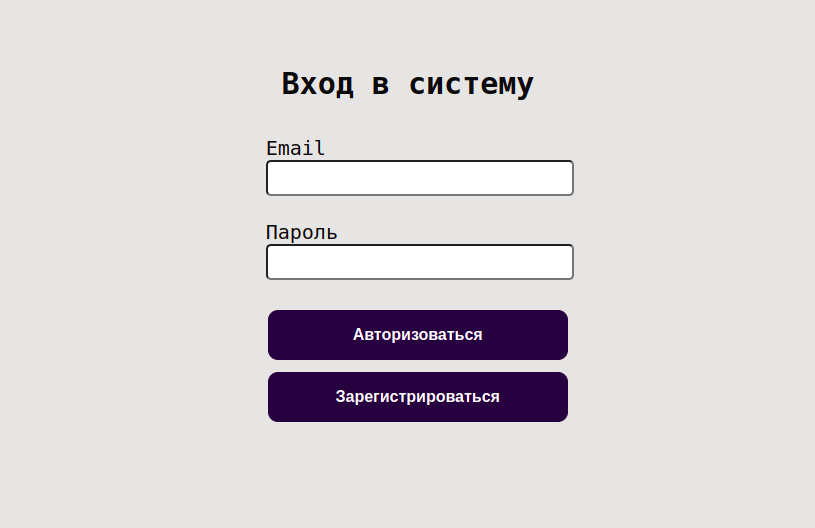
\includegraphics[scale=0.44]{assets/start.png}}
	\caption{Стартовая страница приложения}
\end{figure}

%Т.к. главная страница ориентирована на клиентов (пациентов), то через эту форму может зарегистрироваться только пациент, однако войти может пользователь с любой ролью. 

На рисунке 3.2 представлена форма регистрации для пациента. Формы регистрации, соответствующие ролям <<Доктор>> и <<Администратор>>, будут иметь аналогичный вид.

\begin{figure}[!h]
	\center{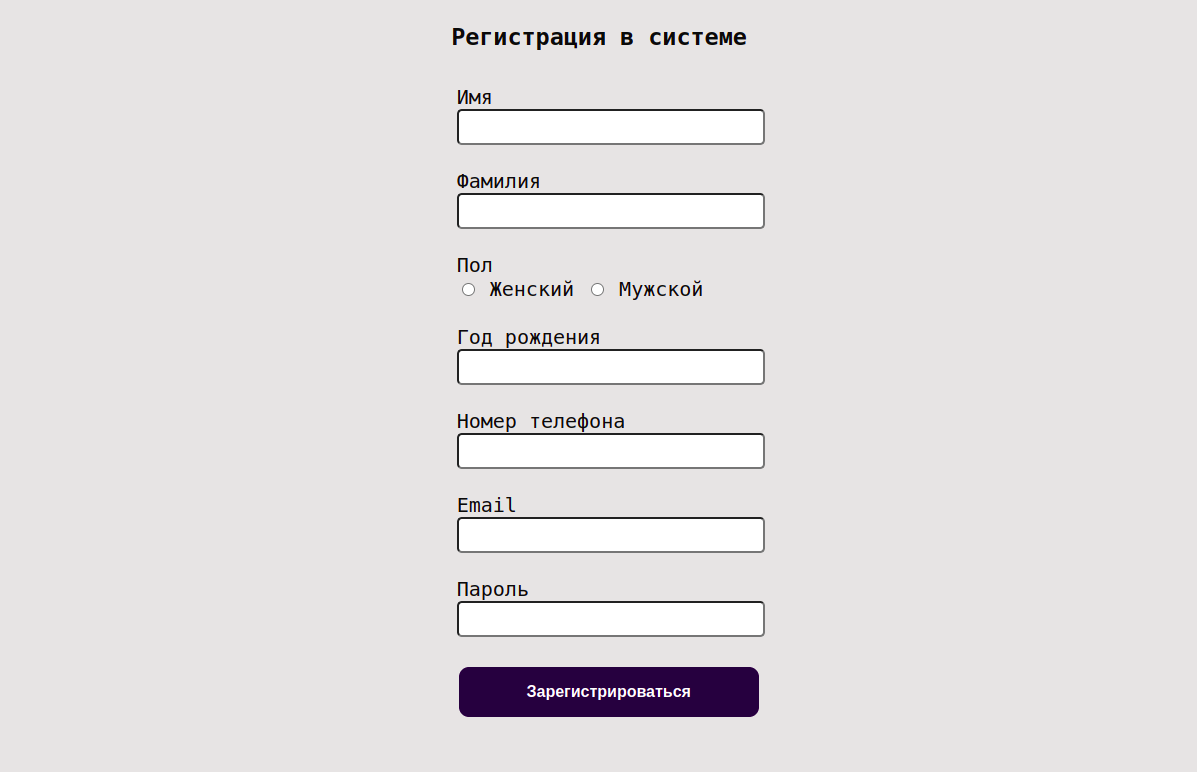
\includegraphics[scale=0.3]{assets/create_patient.png}}
	\caption{Форма регистрации для пациента}
\end{figure}

%На рисунке 3.3 представлена стартовая страница для получения доступа к функционалу регистрации и авторизации администратора. 
%
%\begin{figure}[!h]
%	\center{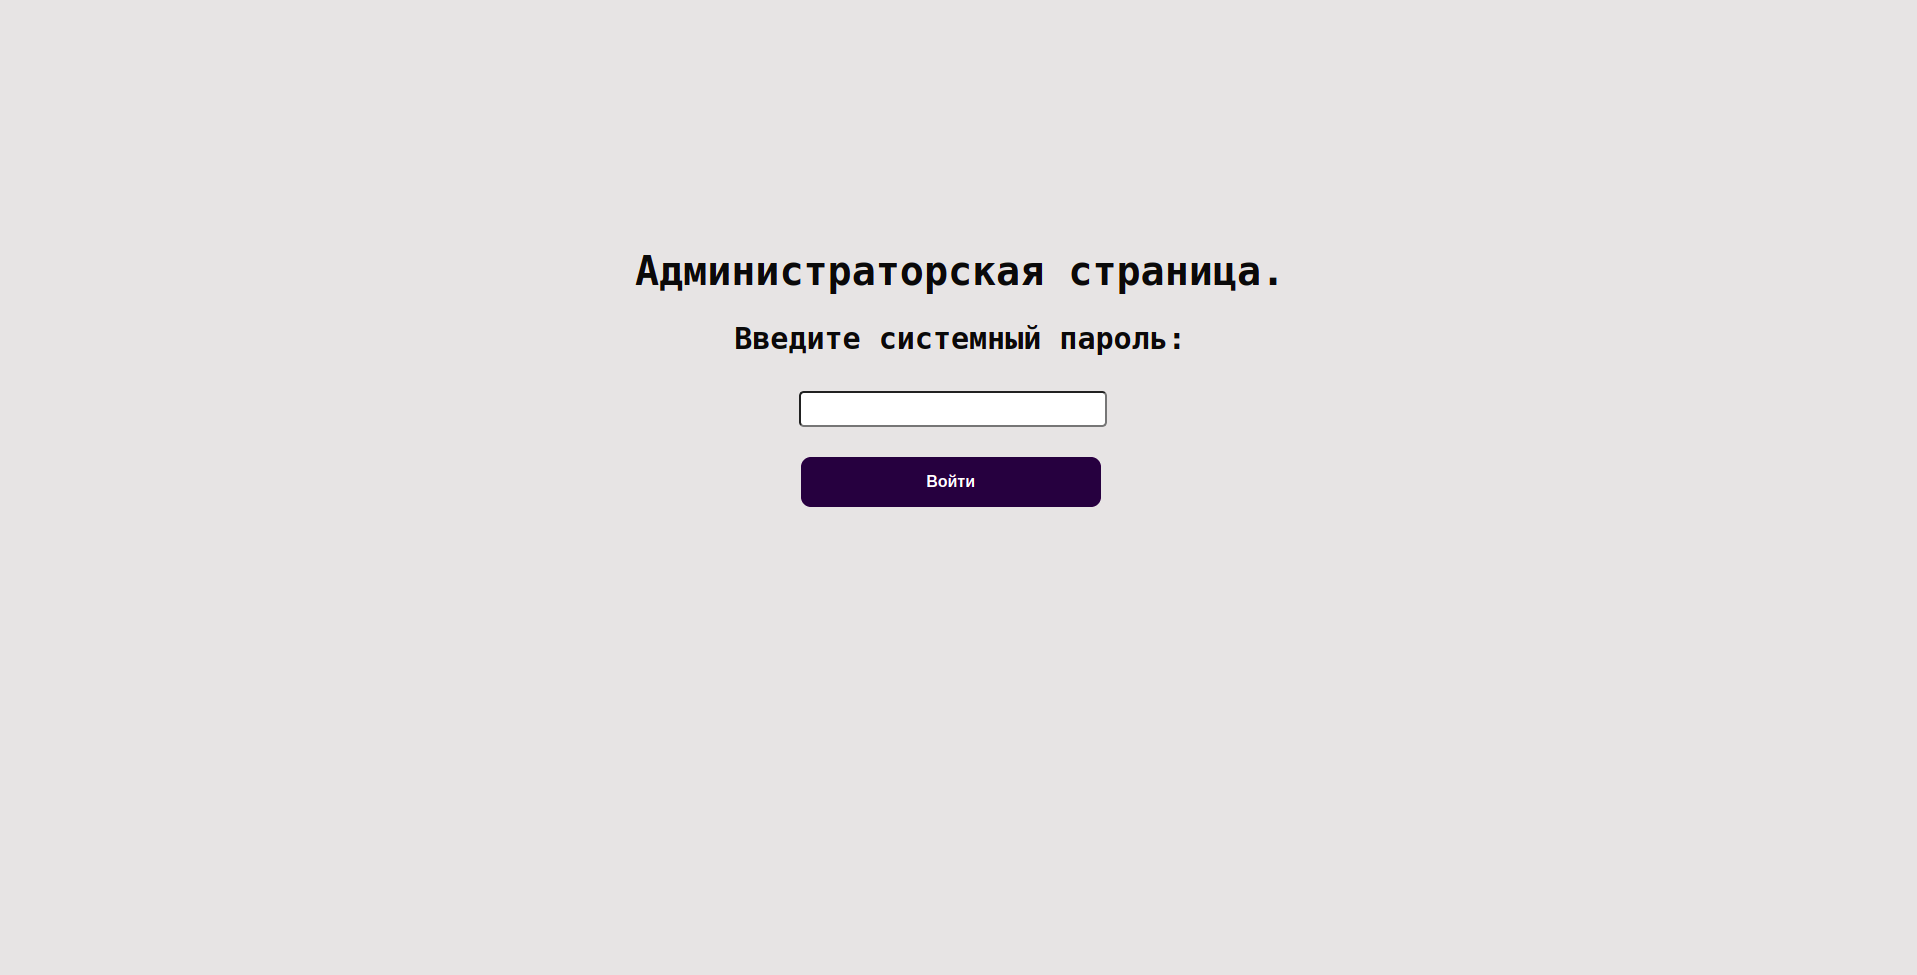
\includegraphics[scale=0.25]{assets/admin_start.png}}
%	\caption{Стартовая страница приложения для администратора}
%\end{figure}
%
%Для начала необходимо ввести системный пароль для подтверждения базовых прав администратора.
%
%На рисунке 3.4 представлен страница, открываемая после успешного ввода системного пароля.
%
%\begin{figure}[!h]
%	\center{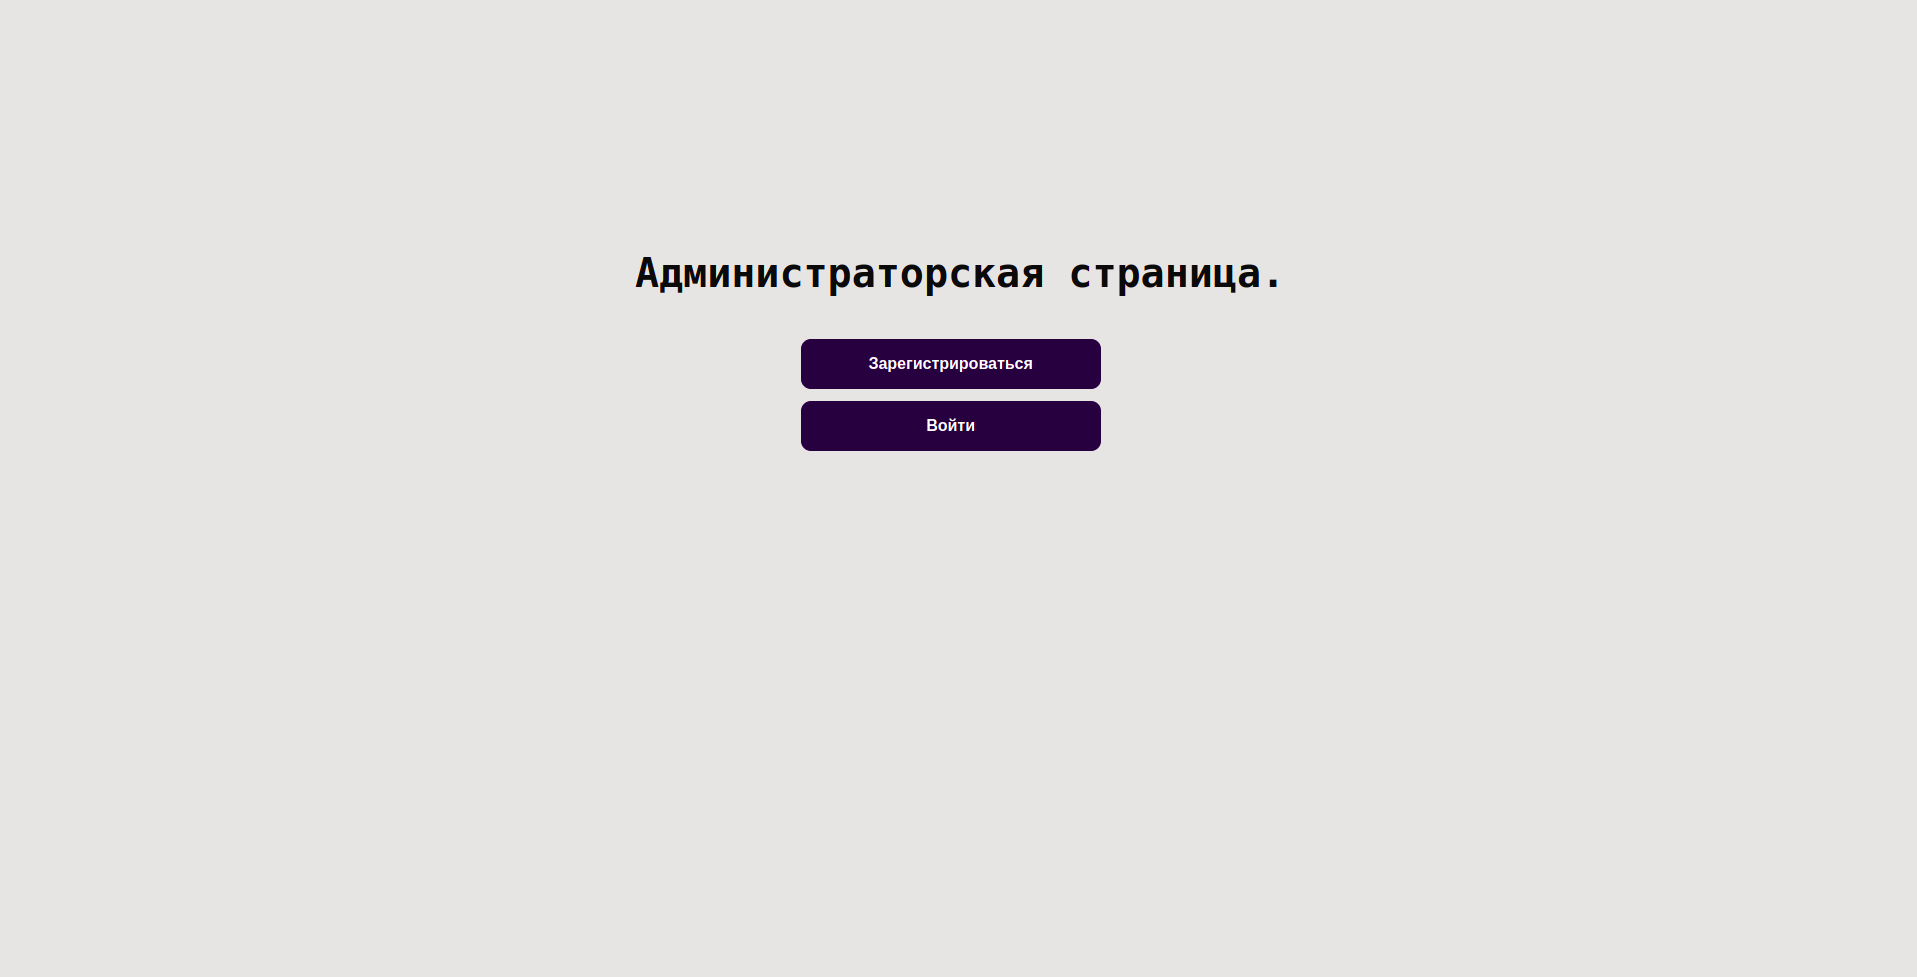
\includegraphics[scale=0.25]{assets/admin_pass.png}}
%	\caption{Стартовая страница приложения для подтвержденного администратора}
%\end{figure}

Для регистрации администратора нужно перейти по специальной ссылке: admin\_start. Зарегистрировать доктора может только администратор.

На рисунке 3.3 представлена страница, демонстрирующая меню авторизированного пользователя с ролью <<Пациент>>.

\begin{figure}[!h]
	\center{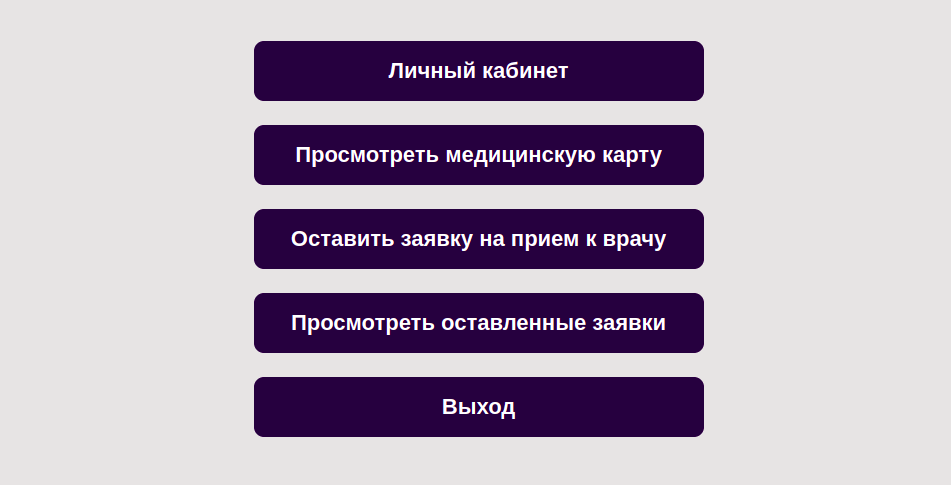
\includegraphics[scale=0.42]{assets/patient_main.png}}
	\caption{Главная страница пациента}
\end{figure}

На рисунке 3.4 представлена страница, демонстрирующая меню авторизированного пользователя с ролью <<Администратор>>.

\begin{figure}[!h]
	\center{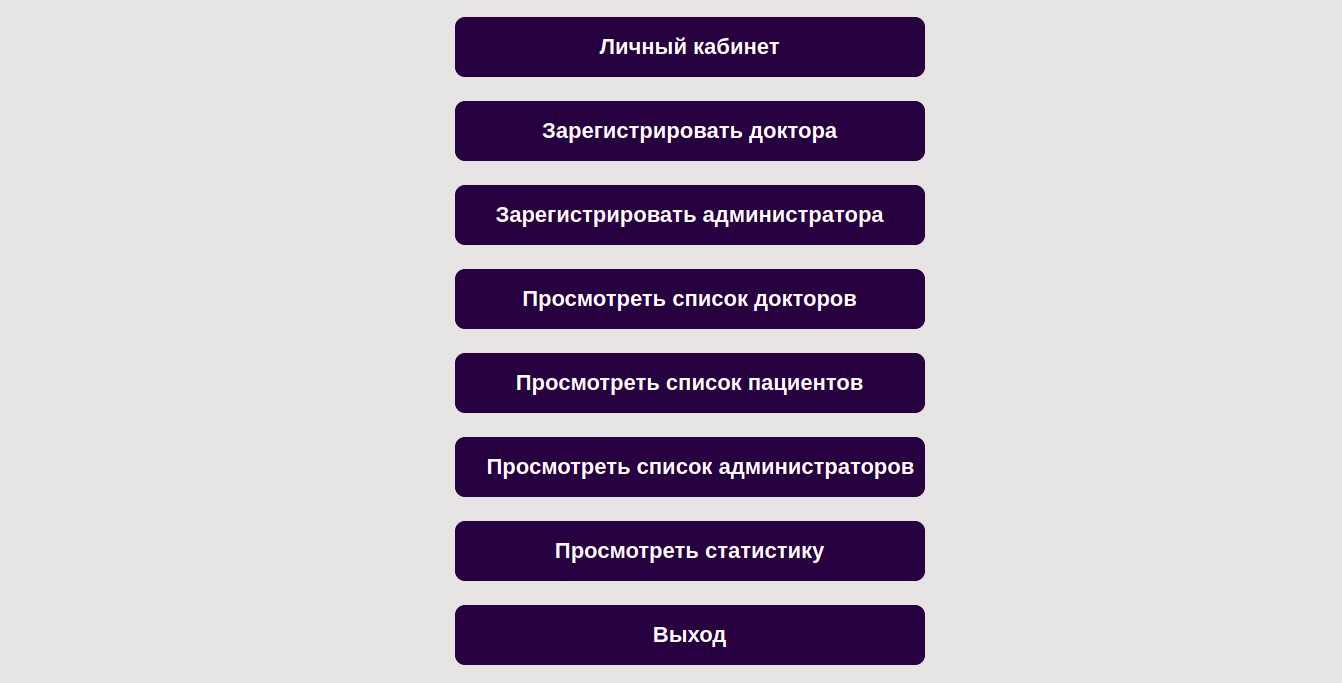
\includegraphics[scale=0.3]{assets/admin_main.png}}
	\caption{Главная страница администратора}
\end{figure}

\clearpage
На рисунке 3.5 представлена страница, демонстрирующая меню авторизированного пользователя с ролью <<Доктор>>.

\begin{figure}[!h]
	\center{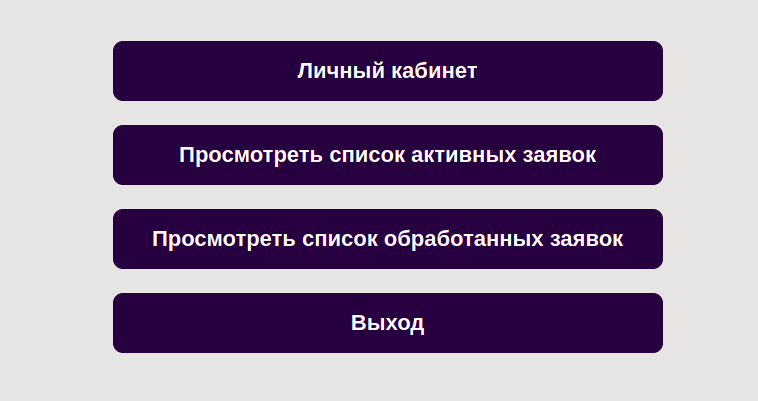
\includegraphics[scale=0.53]{assets/doctor_main.png}}
	\caption{Главная страница доктора}
\end{figure}

На рисунке 3.6 представлена страница, демонстрирующая личный кабинет пользователя с ролью <<Пациент>>.

\begin{figure}[!h]
	\center{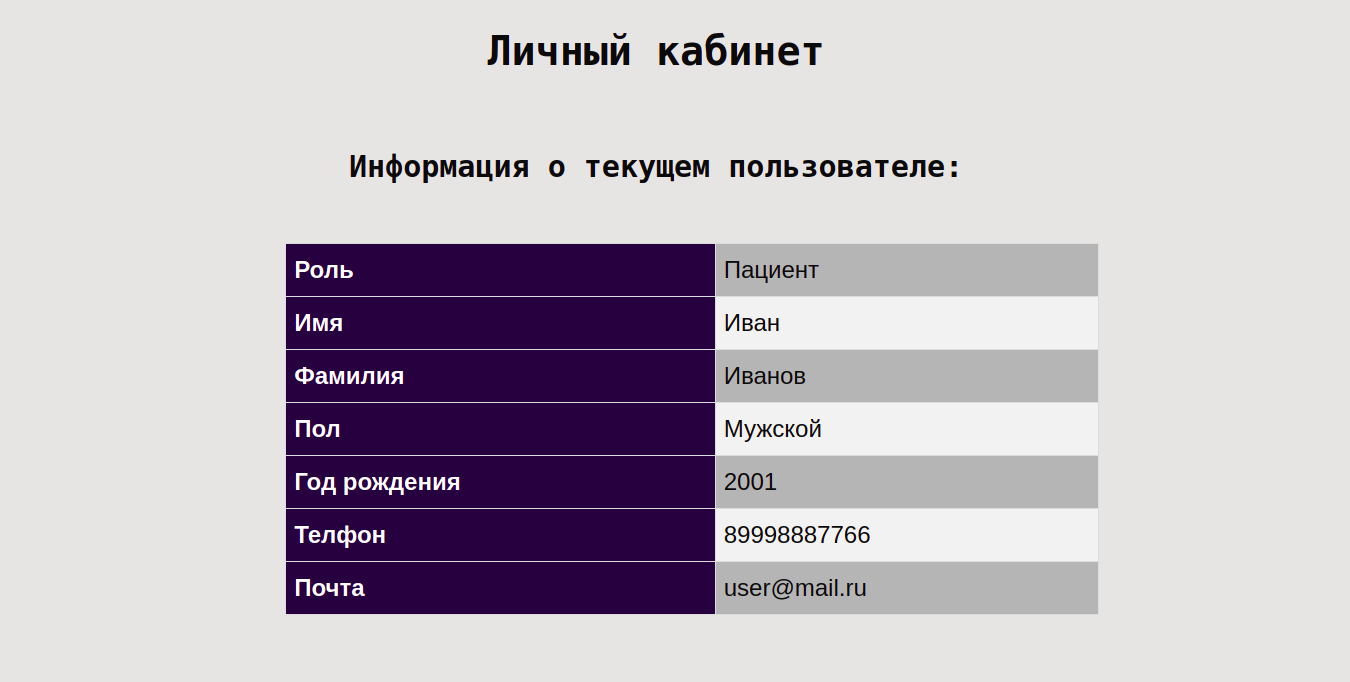
\includegraphics[scale=0.3]{assets/patient_cabinet.png}}
	\caption{Личный кабинет пациента}
\end{figure}

Для пользователей с ролями <<Доктор>> и <<Администратор>> личный кабинет имеет аналогичный вид.

\clearpage

На рисунке 3.7 представлена страница, демонстрирующая медицинскую карту пациента.

\begin{figure}[!h]
	\center{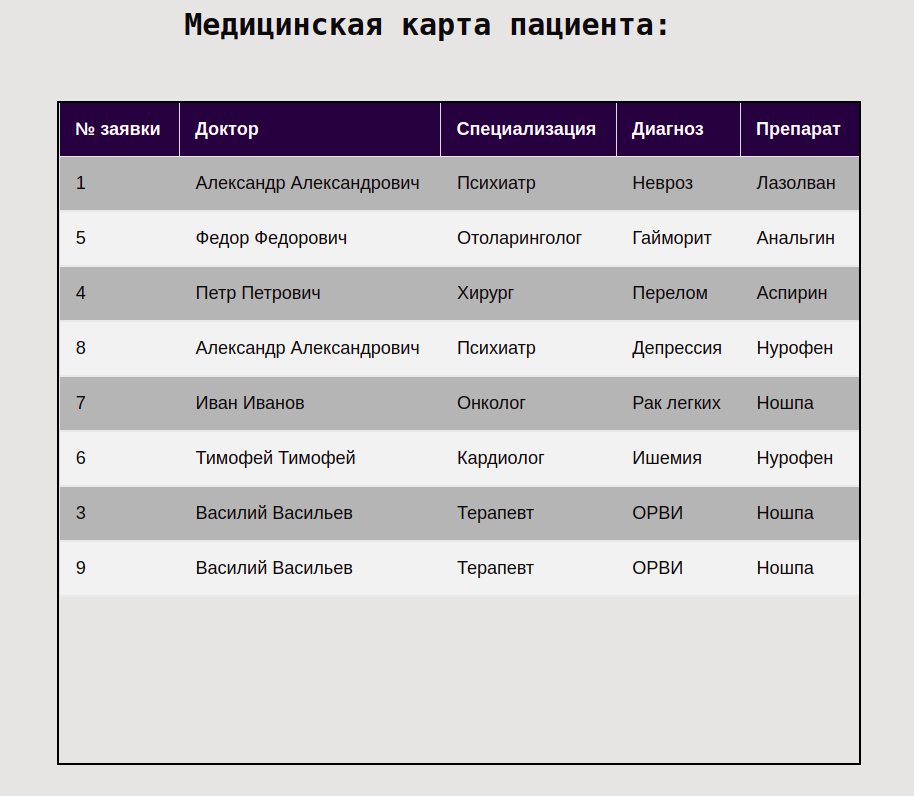
\includegraphics[scale=0.39]{assets/record.png}}
	\caption{Медицинская карта пациента}
\end{figure}

На рисунке 3.8 представлена страница, демонстрирующая форму заявки на прием к доктору.

\begin{figure}[!h]
	\center{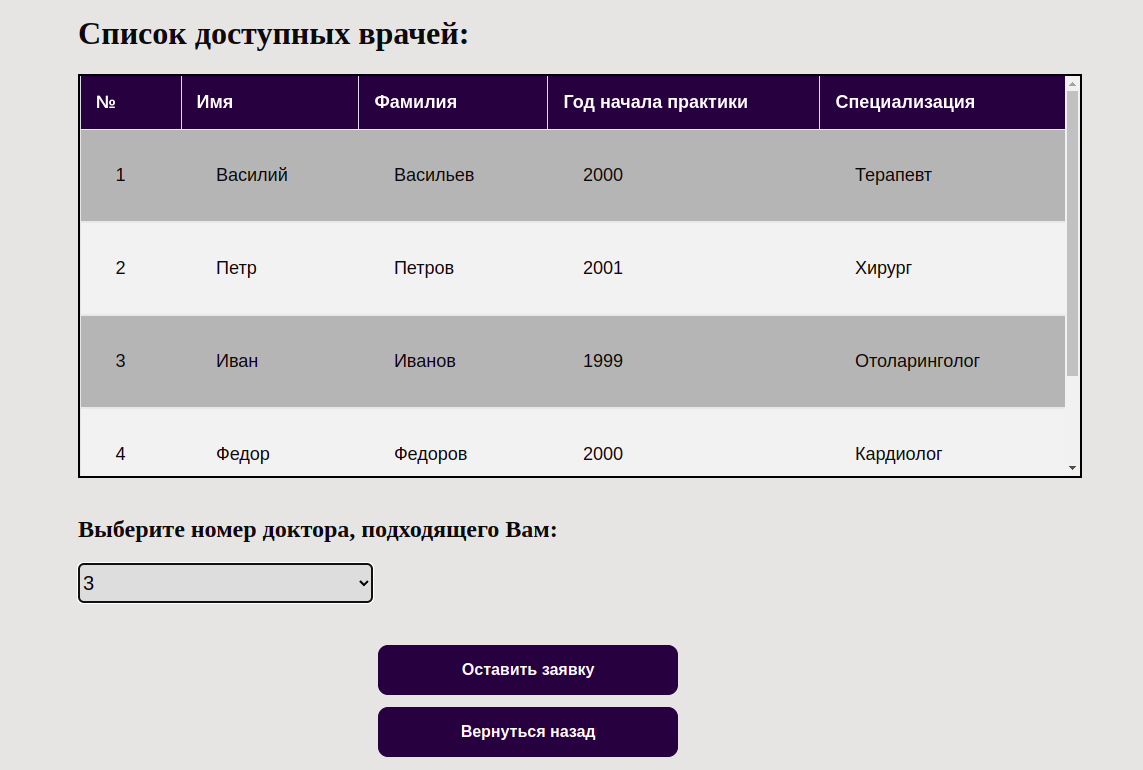
\includegraphics[scale=0.31]{assets/reg_visit.png}}
	\caption{Форма заявки на прием к доктору}
\end{figure}

\clearpage

На рисунке 3.9 представлена страница, демонстрирующая список докторов в системе, доступный только администратору. Страница просмотра списка администраторов и пациентов имеет аналогичный вид.

\begin{figure}[!h]
	\center{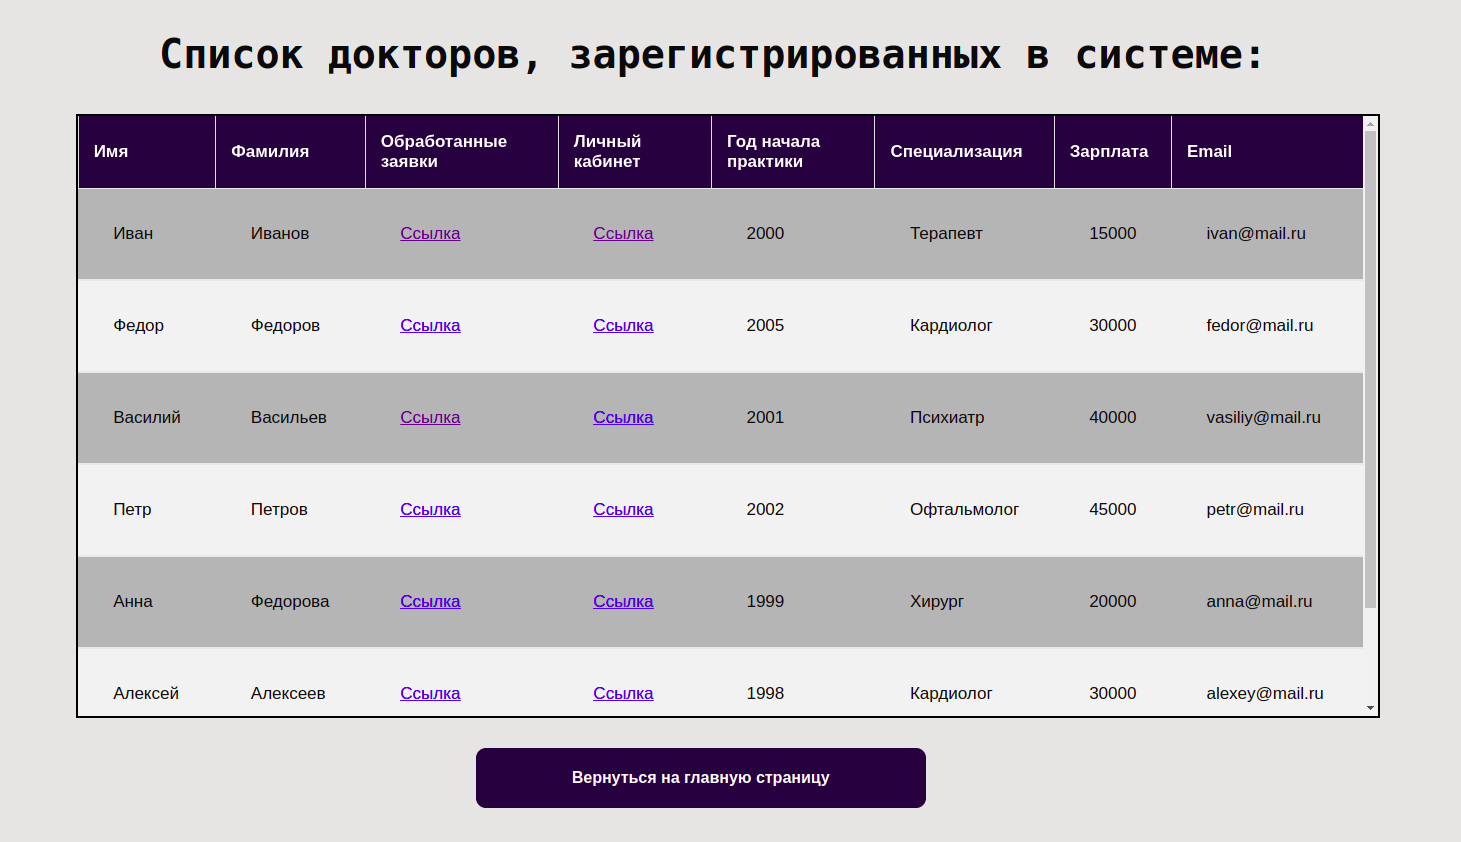
\includegraphics[scale=0.27]{assets/list_doctors.png}}
	\caption{Просмотр списка докторов с системе}
\end{figure}

На рисунке 3.10 представлена страница, демонстрирующая список активных заявок доктора.

\begin{figure}[!h]
	\center{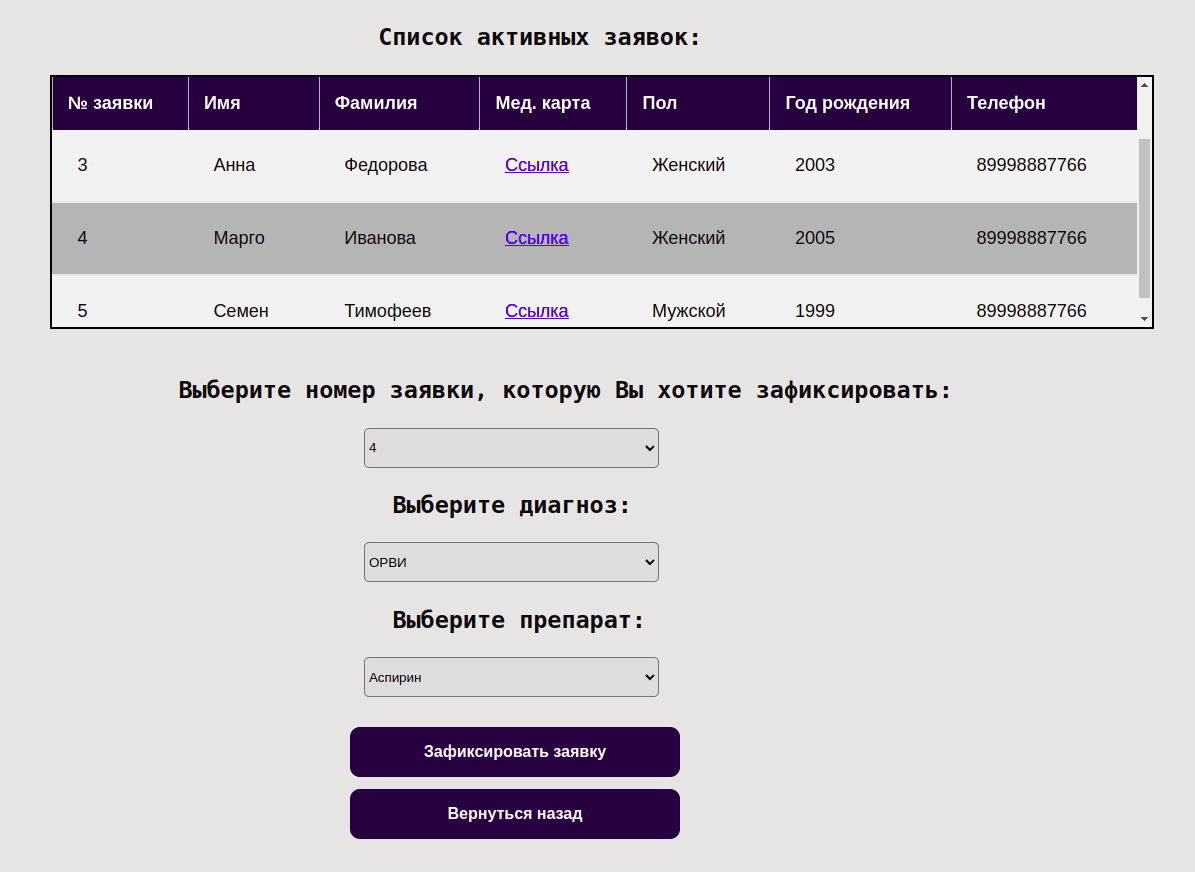
\includegraphics[scale=0.33]{assets/active_visits.png}}
	\caption{Просмотр списка активных заявок доктора}
\end{figure}

\clearpage

На рисунке 3.11 представлена страница, демонстрирующая список обработанных заявок доктора.

\begin{figure}[!h]
	\center{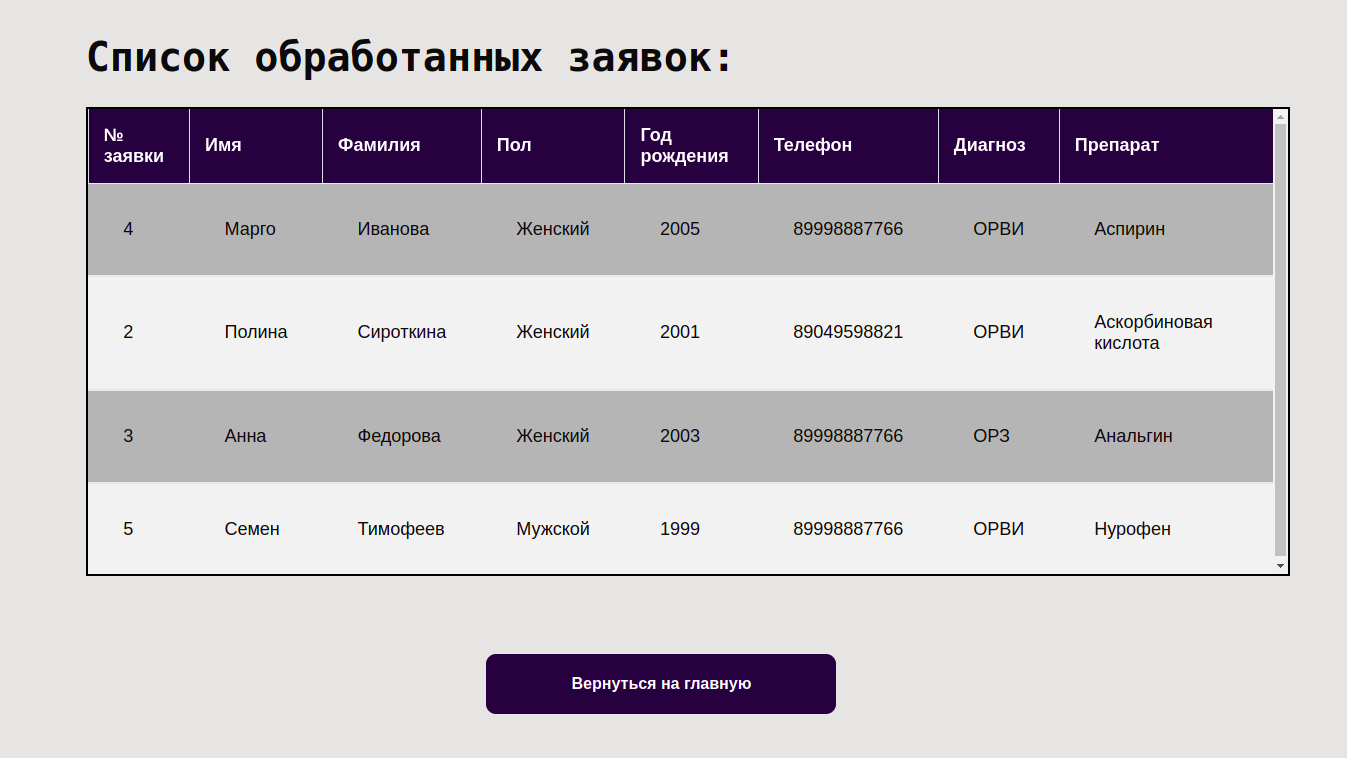
\includegraphics[scale=0.28]{assets/done_visits.png}}
	\caption{Просмотр списка обработанных заявок доктора}
\end{figure}

На рисунке 3.12 представлена страница, демонстрирующая статистику заболеваемости.

\begin{figure}[!h]
	\center{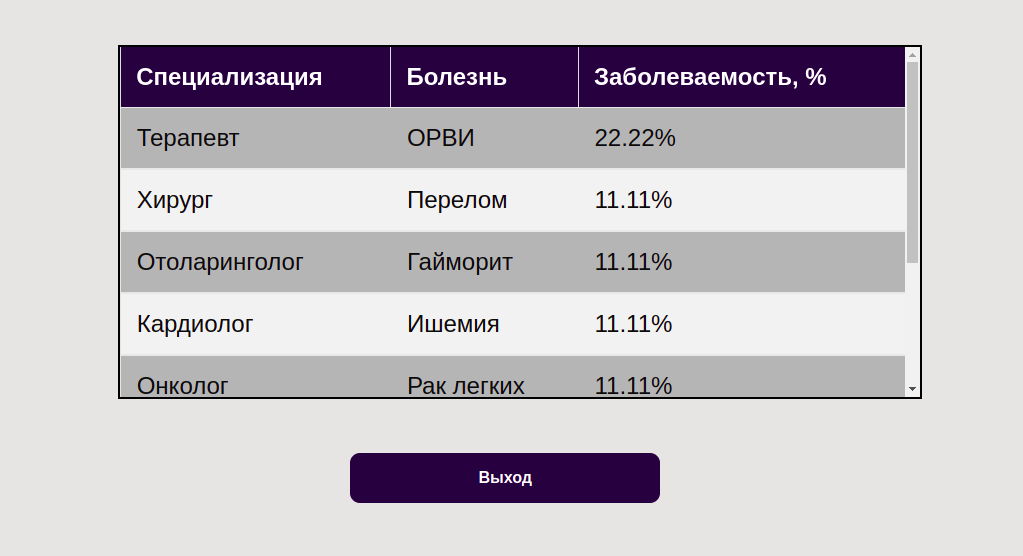
\includegraphics[scale=0.37]{assets/stat.png}}
	\caption{Просмотр статистики заболеваемости}
\end{figure}

\section*{Вывод}

В данном разделе был обоснован выбор средств разработки приложения, представлены детали разработки и дано описание презентационного уровня приложения. Также проведено тестирование приложения.